\begin{wrapfigure}[5]{l}{4cm}
  \centering
  \vspace{-5mm}
  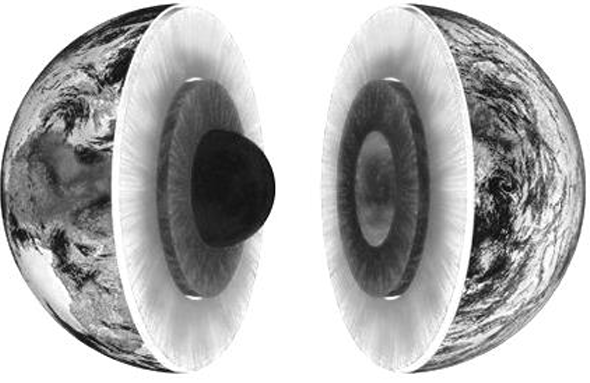
\includegraphics[width=0.2\textwidth]{Figures/P2/Fig 2.1.png}
\end{wrapfigure}

\noindent Cho đến hiện nay, lý thuyết về sự hình thành và tồn tại của từ trường Trái Đất vẫn chưa được hoàn thiện. Trong bài này, ta sẽ phân tích một mô hình đơn giản, qua đó có thể mô tả sơ bộ sự hình thành của từ trường nhờ hiệu ứng máy phát điện từ tính.\\
\indent Từ trường Trái Đất có nguồn gốc từ sự hiện diện của một lớp sắt nóng chảy dẫn điện tốt bên trong lõi Trái Đất và sự tự quay của Trái Đất quanh trục của nó . Xét mô hình sau: một lớp mỏng hình trụ được làm bằng vật liệu dẫn điện quay quanh trục đối xứng của nó với vận tốc góc không đổi $\omega$. Gọi bán kính trong của lớp này là $R$ và độ dày của nó là $h$ với $h\ll R$. Vật liệu làm nên lớp trụ có điện trở suất $\rho$, hằng số điện môi và hằng số từ môi $\varepsilon=\mu=1$. Lớp trụ này được đặt trong môi trường không dẫn điện.\\
\begin{wrapfigure}{r}{4cm}
  \centering
  \vspace{-0.6cm}
  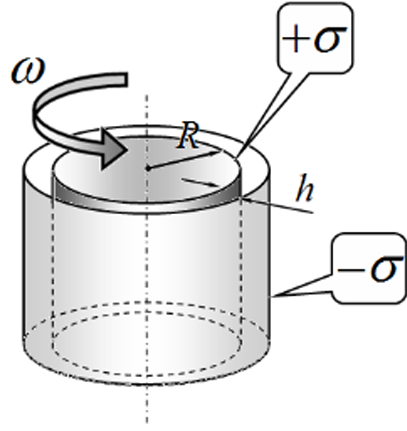
\includegraphics[width=0.2\textwidth]{Figures/P2/Fig 2.2.png}
\end{wrapfigure}

\vspace{-0.4cm}
\indent Ý tưởng chính của việc tạo nên từ trường như sau: Giả sử mặt trong của lớp trụ xuất hiện các điện tích với mật độ điện tích mặt $+\sigma$, khi đó mặt bên ngoài sẽ xuất hiện các điện tích trái dấu với mật độ $-\sigma$. Khi lớp trụ quay, các điện tích này sẽ tạo ra từ trường, tác động lên các electron dẫn, từ đó tạo ra dòng điện giữa mặt trong và mặt ngoài lớp trụ, việc này sẽ làm tăng điện tích tích tụ ở hai mặt nhờ đó gia tăng từ trường.
\subsection*{Phần 1: Trường bên trong lớp trụ}
\begin{wrapfigure}{r}{5cm}
  \centering
  \vspace{-0.6cm}
  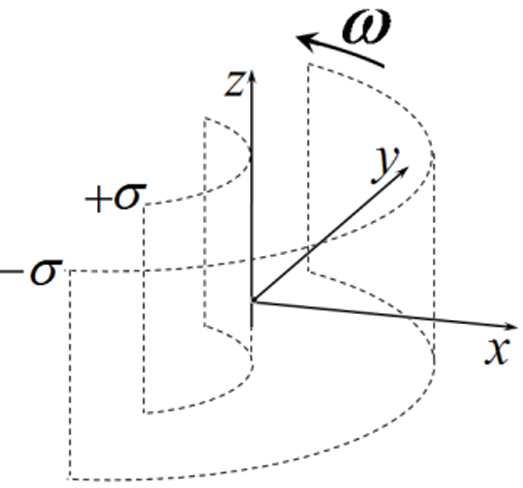
\includegraphics[width=0.25\textwidth]{Figures/P2/Fig 2.3.png}
\end{wrapfigure}

\noindent Để mô tả hiện tượng đang xét, ta sẽ sử dụng một hệ toạ độ Descartes như sau:
\begin{itemize}
  \item Trục $x$ có phương xuyên tâm, vuông góc với các mặt bên của lớp trụ;
  \item Trục $y$ có phương tiếp tuyến với mặt trong của lớp trụ, vuông góc với trục đối xứng của hệ;
  \item Trục $z$ song song với trục đối xứng của lớp trụ;
  \item Gốc toạ độ nằm trên mặt trong của lớp trụ.
\end{itemize}
thực hiện các yêu cầu sau:
\begin{enumerate}
  \item Chỉ ra hướng của các vector: cường độ điện trường $\vec{E}$, cảm ứng từ $\vec{B}$, vận tốc chuyển động $\vec{v}$ của một điểm nằm trong lớp trụ.
  \item Xác định độ lớn cảm ứng từ $B$ tại một điểm nằm trong lớp trụ theo $\sigma,\omega$ và $R$.
  \item Chỉ ra hướng của các lực tác dụng lên các electron dẫn trong lớp: lực $\vec{F}_{E}$ do điện trường tác dụng và lực $\vec{F}_{B}$ do từ trường tác dụng.
  \item Xác định độ lớn các lực $\vec{F}_{E}$ và $\vec{F}_{B}$.
\end{enumerate}

\subsection*{Phần 2: Điện tích và dòng điện}
\noindent Trong phần này, ta sẽ bỏ qua khối lượng của các electron.
\begin{enumerate}
  \item Xác định biểu thức mô tả sự phụ thuộc của độ biến thiên mật độ điện tích mặt $\Delta\sigma$ theo thời gian $\Delta t$. Biểu thức này chỉ được chứa các thông số của lớp trụ và các hằng số vật lý.
  \item Xác định tốc độ chuyển động tới hạn của lớp $V^{*}=\omega R$ ở đó nếu tốc độ của lớp vượt qua giá trị này thì từ trường trong lớp có thể tăng theo thời gian. Áp dụng bằng số: $R=3,5.10^{6}\,\SI{}{\ohm}$, $\rho=1,4.10^{-6}\,\SI{}{\ohm\metre}$.
  \item Tích độ dài một ngày trên Trái Đất trong trường hợp tốc độ chuyển động của lớp đạt giá trị tới hạn.
  \item Giả sự mật độ điện tích mặt trên bề mặt của lớp trụ tại một thời điểm nào đó bằng $\sigma_{0}$. Ước tính thời gian đặc trưng để các điện tích này biến mất nếu tốc độ quay của lớp bằng tốc độ quay của Trái Đất.
\end{enumerate}

\subsection*{Phần 3: Khối lượng của electron có cứu mô hình này không?}
\noindent Khác với phần trước, trong phần này ta sẽ xét tới khối lượng của các electron $m_{e}=9,1.10^{-31}\SI{}{\kilogram}$. Giả sử lớp trụ quay với tốc độ góc bằng tốc độ góc của Trái Đất.
\begin{enumerate}
  \item CHứng minh rằng khi xét đến khối lượng của các electron, tồn tại các điện tích đứng yên trên các bề mặt của lớp trụ. Xác định mật độ điện tích mặt của các điện tích này.
  \item Tính cảm ứng từ bênt trong lớp trụ trong trường hợp này. So sánh kết quả của bạn vói cảm ứng từ trung bình trên bề mặt Trái Đất $B_{0}\approx\SI{40}{\micro\tesla}$.
  \item Dựa vào các kết quả của bạn, hãy đưa ra kết luận: liệu mô hình này có thể mô tả cơ chế hình thành từ trường của Trái Đất không?
\end{enumerate}